\def\Title{\hfill \huge{変化する社会への適応力を涵養する著作権法の教育実践} \hfill}
\def\Author{大西 洋 (京都市立西京高校)}
\include{myposter}
\include{embed}
\definecolor{em-bg}{rgb}{0.8, 1.0, 0.8}

\bibliography{poster-zen2017}
\nocite{*}
\Header

\section{Background}
\begin{columns}[onlytextwidth,t]
\begin{column}{.35\hsize}
\begin{block}{\insertsection}
\alert{法令}: \em{社会のルール}
\begin{itemize}
\item[⇨] 本来は\em{義務教育終了時点で読めるべき}もの
\item 社会科・公民科: 憲法しか扱わない(ことが多い)
\item 教科書: 現行or古い法の条文を\em{「解説」}
\item[⇨] \em{数年で変わる}現行法の「解説」に意味はある? \\
	次はクラウドストレージ? フェアユース?
\item 巻末付録: 省略が多く不十分
\item[⇨] 親告罪規定は載っている?
\end{itemize}
\end{block}
\end{column}
\begin{column}{.45\hsize}
\begin{block}{近年の著作権法改正(抄)}
著作権法は\alert{頻繁}に、かつ\alert{身近な部分}が改正される\cite{hourei}
\begin{itemize}
\item \em{2010}/1: H21法律第53号 (2009/6) \\
	キャッシュ保存権利制限, \em{オークション}用写真掲載, \\
	\em{違法アップロードの録音/録画}違法化, 点訳等権利制限
\item \em{2012}/10: H24法律第43号 (2012/6) \\
	\em{違法ダウンロード}刑罰化, \em{「写り込み」}, \em{DRM回避}違法化
\item ??/??: H28法律第108号 (2016/12) \\
	\alert{TPP}(\em{非親告罪化}, \em{保護期間延長}), \em{アクセス制限回避}違法化
\end{itemize}
\end{block}
\end{column}
\begin{column}{.15\hsize}
\begin{block}{法律の構成\cite{sangiin}}
本則
\begin{itemize}
\item 総則的規定
	\begin{itemize}
	\item \alert{目的}(第1条)
	\item \alert{定義}(第2条)
	\end{itemize}
\item 実体的規定
\item 雑則的規定
\item \em{罰則}規定
\end{itemize}
附則
\end{block}
\end{column}
\end{columns}

\begin{columns}[onlytextwidth,t]
\begin{column}{.35\hsize}
\begin{alertblock}{Research Purpose}
\alert{社会の変化}への対応力を涵養できる授業の構築
\begin{itemize}
	\item \em{法令}(\alert{著作権法})を読解する授業を実施
	\item[⇨] 著作権法の\em{条文}を配布
	\item 授業の\em{目的を明示}し動機づけ
	\item グループでの\em{協働学習}による理解の深化
	\item[⇨] \em{実際の場面}に即した\em{演習}問題を作成
	\item 知財や法の時事問題との関連づけ
	\item[⇨] 個人情報保護法の改正など
\end{itemize}
\end{alertblock}
\end{column}
\begin{column}{.35\hsize}
\begin{figure}[hbtp]{\centering
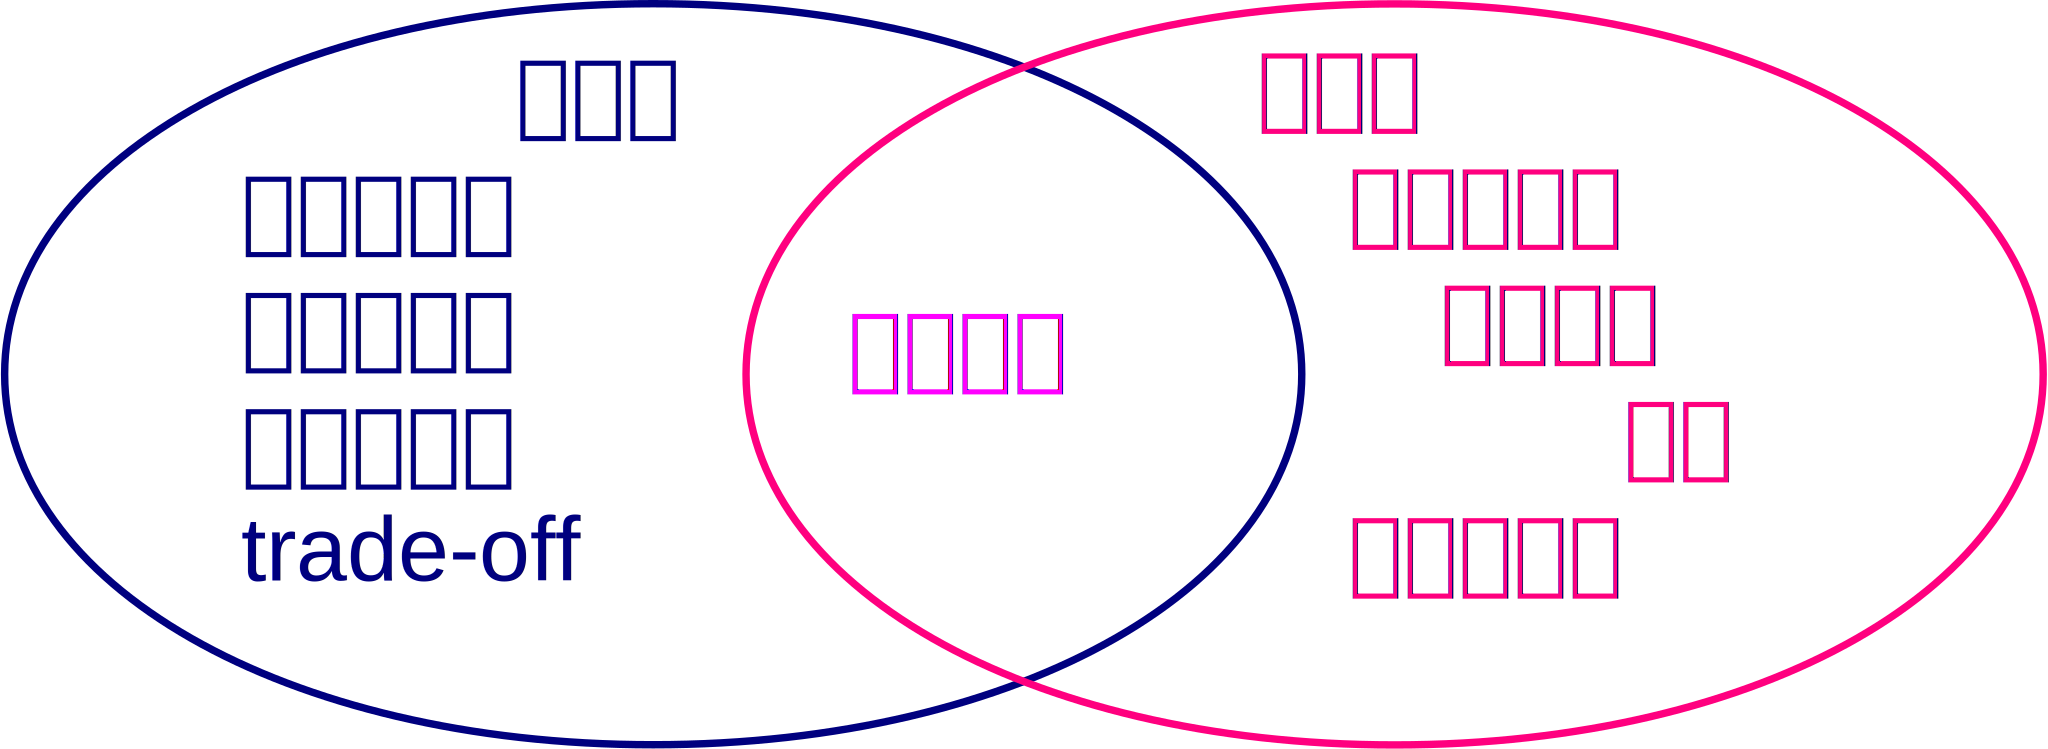
\includegraphics[scale=2.5]{civics_and_informatics.pdf}
\caption{著作権に関連する公民科と情報科の内容}
}\end{figure}
\end{column}
\begin{column}{.27\hsize}
\begin{block}{境界分野としての法教育}
\em{公民}科 or \alert{情報}科: どちらで扱うべき?
\begin{itemize}
	\item \alert{情報}科は\alert{創発}による\em{文化・社会の発展}を扱いたい
	\item[⇨] 望ましいのは\em{公民}科で扱うこと
	\item[⇨] (勤務校の事情) 1年に公民科の授業がない
	\item 「法教育」の実践も法の\em{理念面}が中心
	\item[⇨] 条文読解に焦点化していない
\end{itemize}
\end{block}
\end{column}
\end{columns}


\section{Practice}
\begin{columns}[onlytextwidth,t]
\begin{column}{.35\hsize}
\begin{exampleblock}{\insertsection}
著作権の授業を4年間実践
\begin{itemize}
	\item 対象: 高1, 「\em{情報学基礎}」(学校設定科目)
	\item 5月に2時間連続(50分×2)の授業1回 $+ \alpha$で実施
	\item \em{創発}(emergence)の下位分野として位置づけ \\
		(特許, アイデア, 個性, 水平思考, SCAMPER, \alert{著作権})
\end{itemize}
\end{exampleblock}

\begin{block}{図解の使用}
授業では条文の説明を原則としつつ、文章で捉えにくい関係や構造の理解を促すために\em{図解}を使用
\begin{figure}[hbtp]{\centering
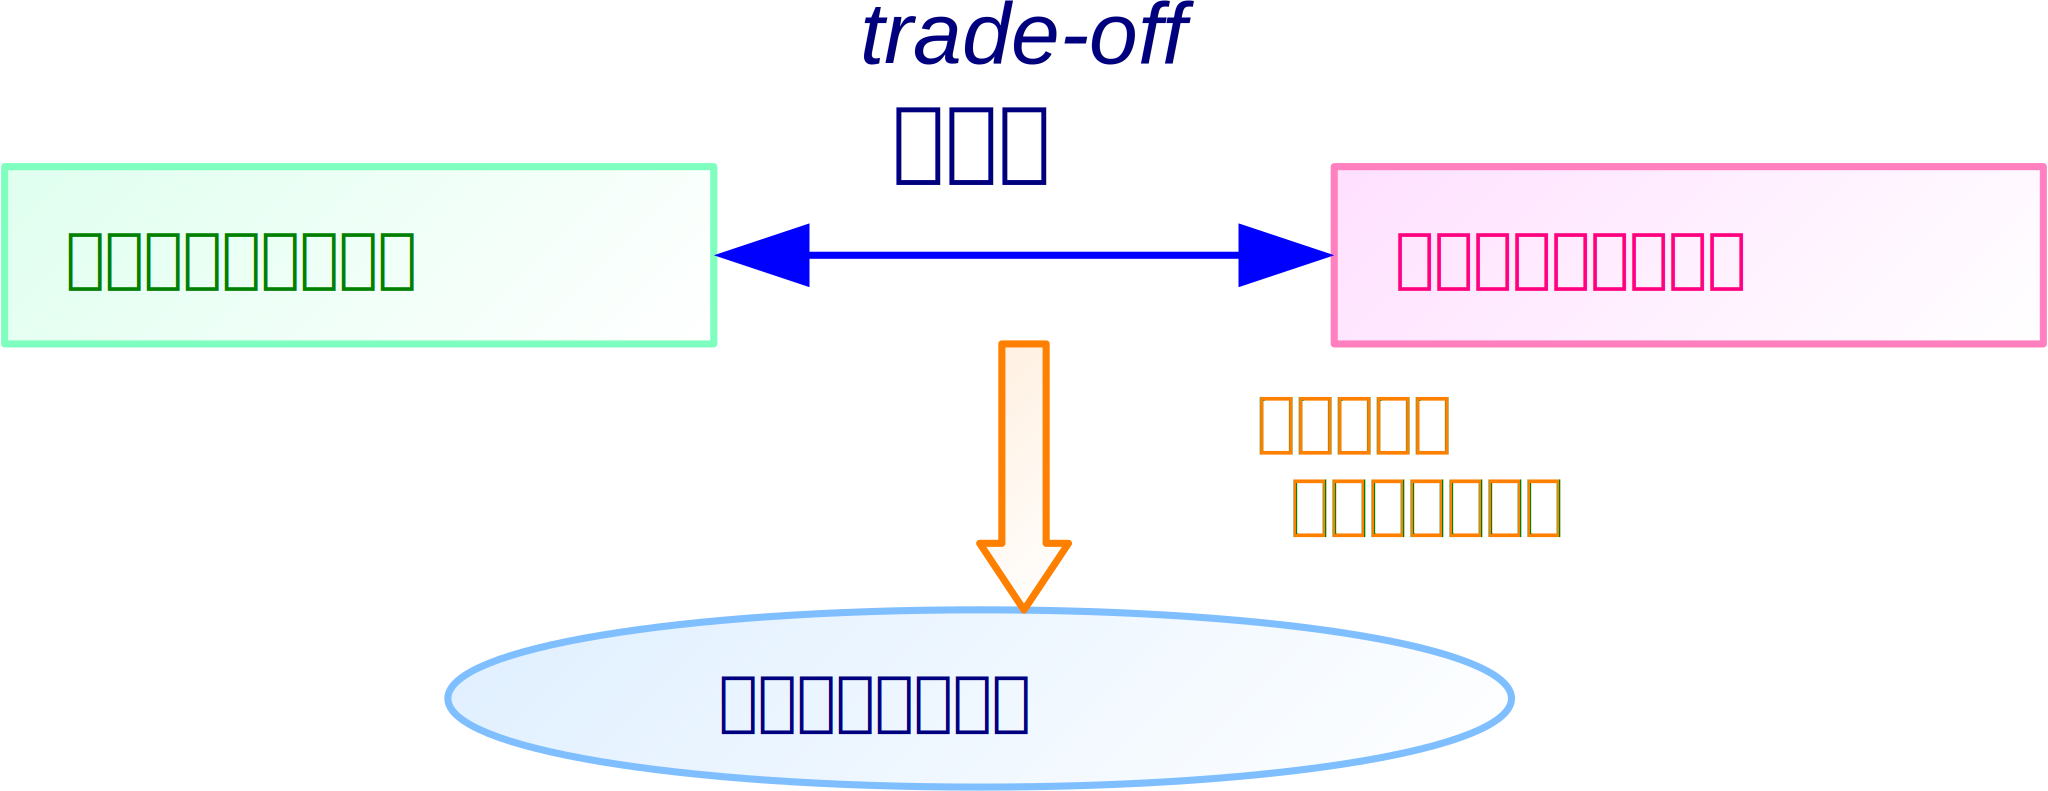
\includegraphics[scale=2.5]{slide-copyright-tradeoff.pdf}
\caption{二者間のtrade-off関係}
}\end{figure}
\begin{figure}[hbtp]{\centering
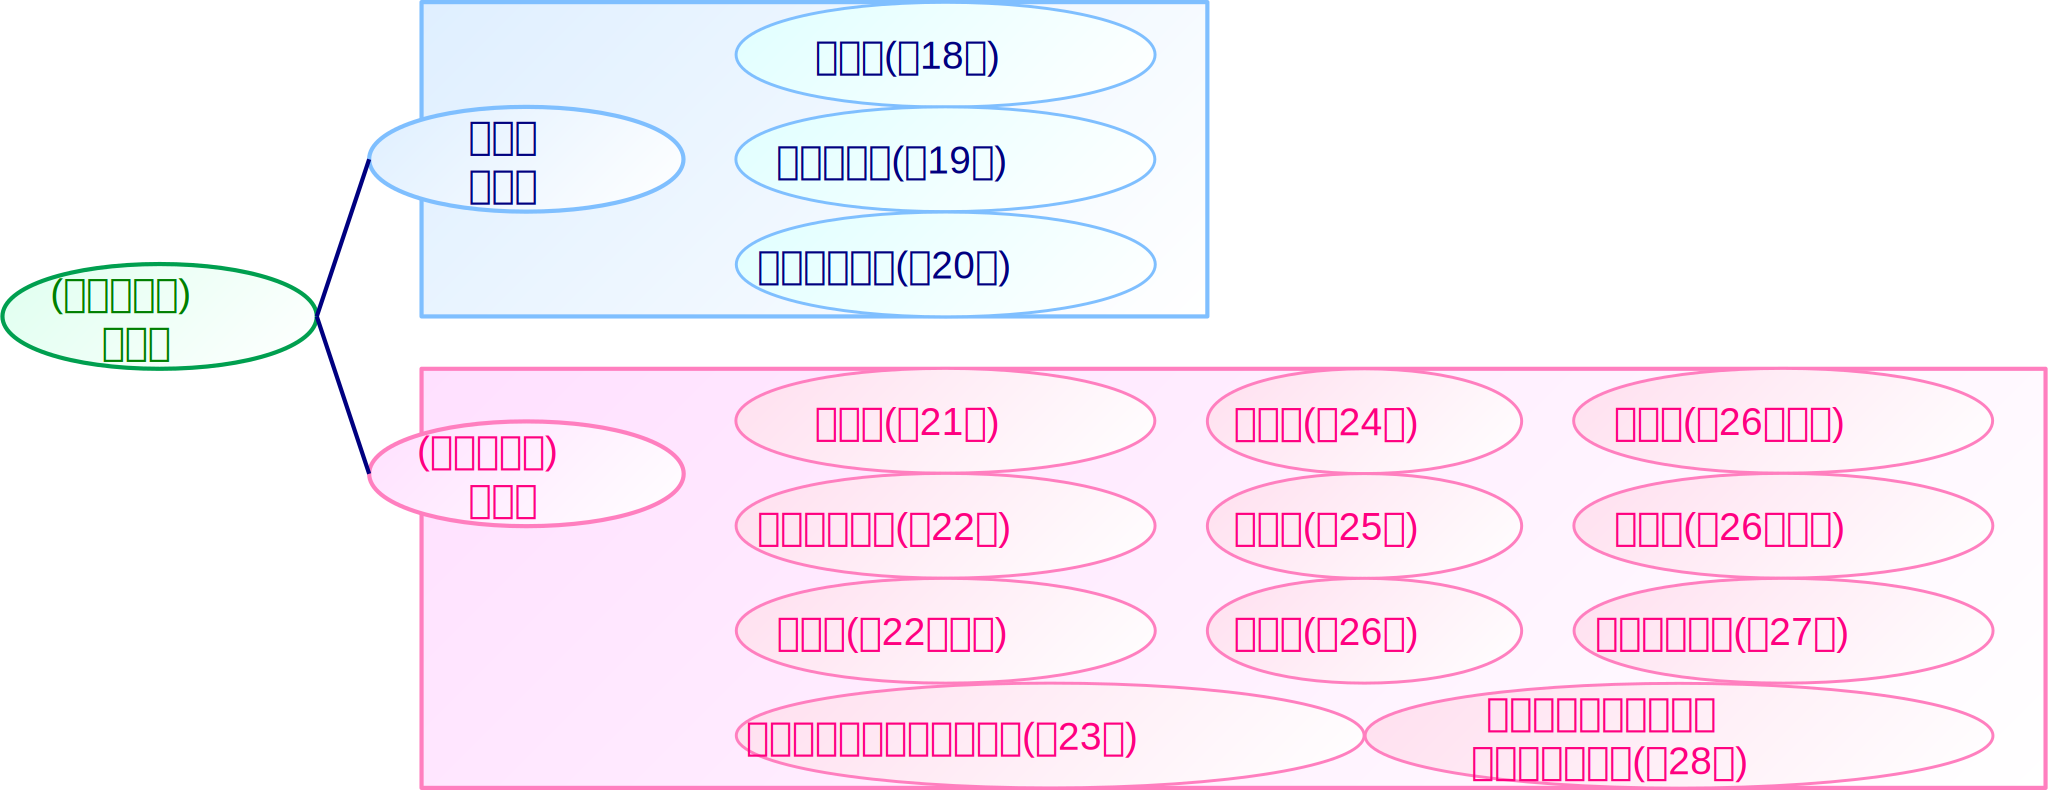
\includegraphics[scale=1.5]{slide-copyright-rights.pdf}
\caption{著作権に含まれる権利}
}\end{figure}
\end{block}

\begin{block}{授業後の定着}
事後にも本時の能力・知識を定着させる取り組みを実施
\begin{itemize}
\item 考査でも知財の問題に時事問題を使用
\item 個人情報の単元で個人情報保護法の条文を配布
\end{itemize}
\end{block}
\end{column}
\begin{column}{.62\hsize}
\begin{block}{授業構成}
演習を挟みながら、説明を中心にして授業を展開
\begin{figure}[hbtp]{\centering
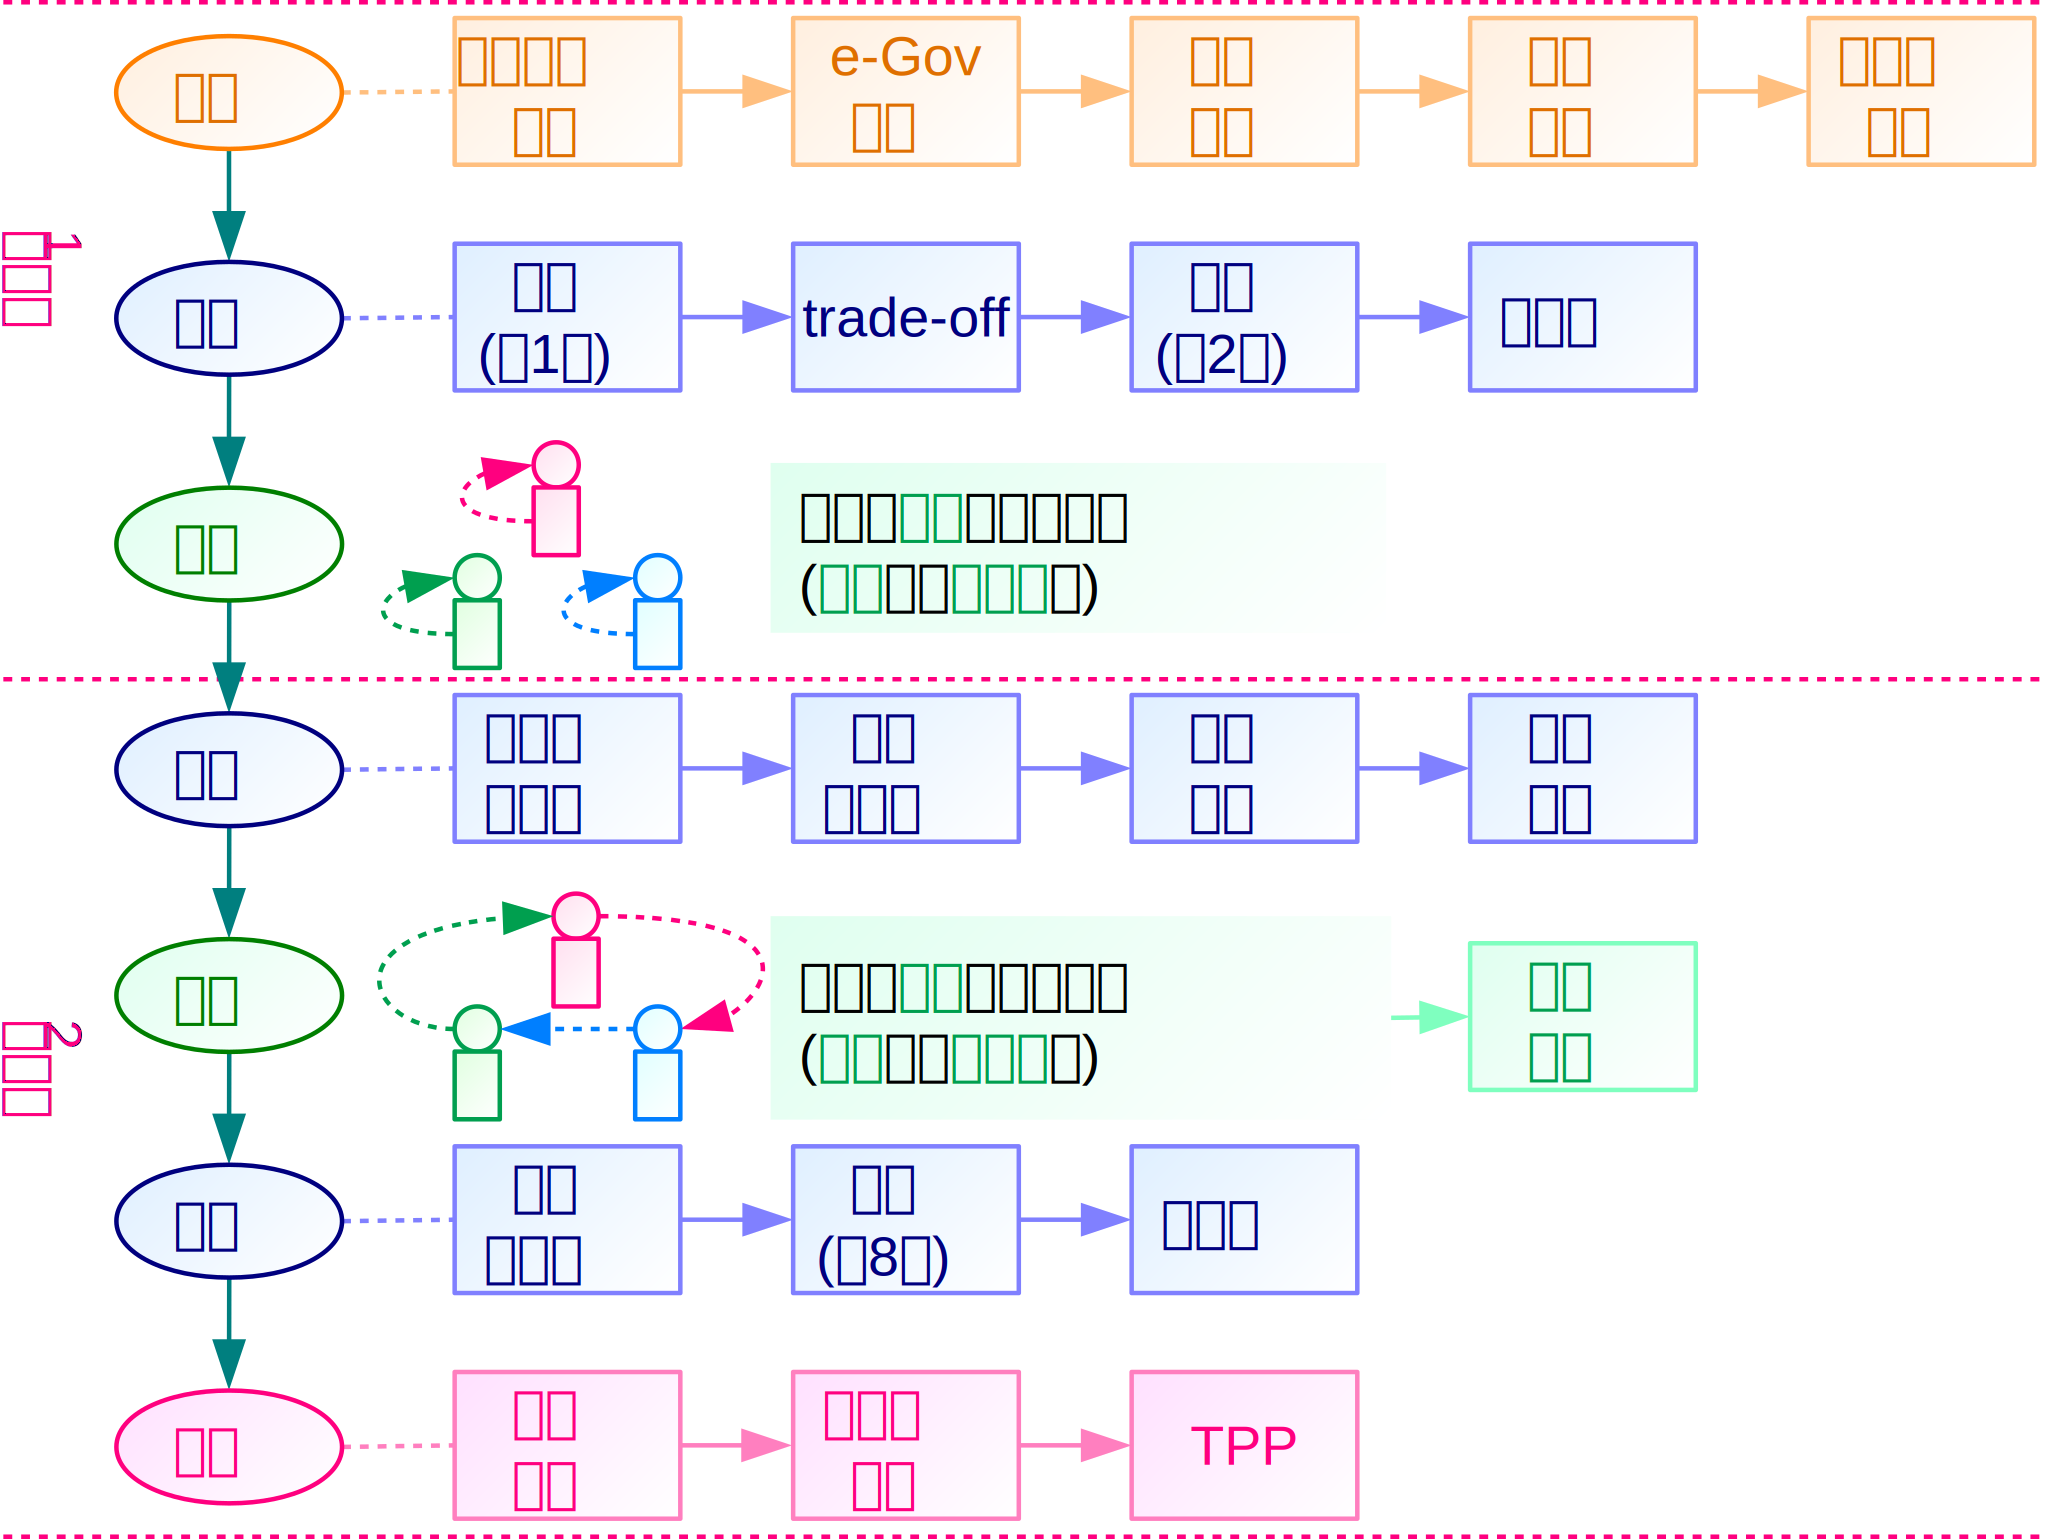
\includegraphics[scale=2.5]{flow.pdf}
\caption{2時間の授業構成}
}\end{figure}
\end{block}

\begin{exampleblock}{演習課題(抄)}
次の行為が著作権法に\em{違反するか}どうか、\em{理由(どの条文が根拠となるか)も含め}班で検討せよ
\begin{itemize}
	\item ディズニーランドの公式サイトからダウンロードしたミッキーマウスの画像の一部を、Twitterのプロフィール画像として使用する行為
	\item 初音ミクのコスプレで街中を歩き、1枚100円の撮影料で通りがかりの人の撮影に応じる行為
	\item レンタルCDショップで借りたCDから音楽を自身のPCやiPod・携帯電話にコピーする行為
	\item 1人500円の参加費をとって、映画「ローマの休日」(1953年公開)の上映会を行う行為
\end{itemize}
\end{exampleblock}
\end{column}
\end{columns}


\section{Conclusion}
\begin{columns}[onlytextwidth,t]
\begin{column}{.35\hsize}
\begin{block}{評価}
\begin{figure}[hbtp]{\centering
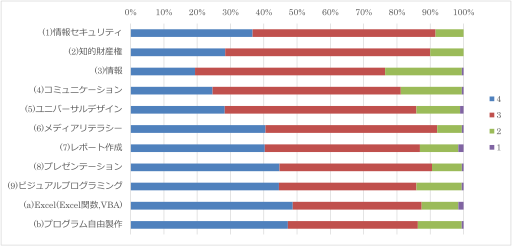
\includegraphics[scale=1.5]{enq.pdf}
\caption{学年末アンケートにおける単元別満足度}
}\end{figure}
\end{block}
\end{column}
\begin{column}{.62\hsize}
\begin{block}{生徒の感想(学年末アンケートより)}
	\begin{itemize}
		\item 著作権に関する学習は、情報がすごく早く行き来する\em{今の社会にすごく必要}な知識だと思うので学べてよかったと思います。
		\item 著作権やセキュリティーなど情報化社会に生きる私たちにとって,とても\em{身近で知る必要がある}内容を学べたのは良かったと思う。
		\item 著作権など\em{知っていないと将来トラブルに巻き込まれそう}なことを知れたのはよかったと思う。
		\item 著作権法に関しては特に近年日本では曖昧になっているところもあるのできちんと学べて良かった。
	\end{itemize}
\end{block}

\begin{block}{Future Tasks}
	\begin{itemize}
		\item 校内での活動を題材とし、\em{協同学習}の比率をより高める
		\item \em{条文読解そのものの効果}を測定する評価の実施
	\end{itemize}
\end{block}

\begin{block}{References}
\renewcommand*{\bibfont}{\scriptsize}
\printbibliography
\end{block}
\end{column}
\end{columns}

\end{frame}
\end{document}
